\documentclass{zpt}
\title{实验二: 语法分析器}
\begin{document}
    \maketitle
    \tableofcontents
    \clearpage
    \section{实验内容}
    用C++实现对给定文法的语法分析器。
    \section{程序设计原理与方法}
    \subsection{原理}
    使用\textbf{LL(1)分析器}
    \begin{itemize}
        \item 对输入字符串进行词法分析, 将其解析为句子
        \item 根据给定文法求各个符号的$\mathsf{First},\mathsf{Follow}$集
        \item 根据$\mathsf{First},\mathsf{Follow}$集求每个文法的$\mathsf{Select}$集
        \item 构造分析表
        \item 进行LL(1)分析
    \end{itemize}

    \subsection{方法}
    明确了原理后, 参照课本和老师给的例子, 进行一步步实现。语法分析器的逻辑甚至比词法分析器还简单, 就是按照上述一步步做就可以了;\par
    由于老师给的文法较为简单, 我认为更加挑战的在于如何写出一个\emph{优雅的}语法分析器, 我使用\textbf{类}来实现, 目的有两个:\begin{enumerate}
        \item 更好地抽象出\textbf{符号, 文法, 分析器}的概念, 方便自己的理解, 以及后续能够方便地引入到别的文件中;
        \item 尽可能少地使用空间, \textbf{多使用指针};
    \end{enumerate}
    具体来说, 我分别定义了如下5个类:
    \begin{lstlisting}[language=c++]
// 符号类
class Symbol{
    public:
        char symbol;                        // 具体符号
        int index;                          // 符号的序号, 对应在最终的分析表中的行号/列号
        bool produce_e;                     // 是否能产生epsilon
        bool is_terminal;                   // 是否是终结符

        Symbol();
        Symbol(char,int,bool);

        set<Symbol*> first;                 // First集
        set<Symbol*> follow;                // Follow集

        int append_first(Symbol*,int);
        int append_follow(Symbol*, int);

        void printFirst();
        void printFollow();
};

// 符号集
class Symbols{
    public:
        Symbols();
        int len();
        void info();                        // 打印符号集中所有符号的相关信息

        void append(Symbol*);               // 给符号集添加新的符号
        Symbol* find(char);                 // 根据符号的值查找某一个符号

        map<char,Symbol*> symbols;          // 用字典保存符号集中符号的指针
};

// 文法类
class Grammer{
    public:
        Grammer();
        Symbol* head;                       // 文法的左式, 直接对应到相应的符号
        string tail;                        // 文法的右式, 由于不止一个符号, 因此还是用字符串保存符号的值

        set<Symbol*> select;                // 文法的select集, 同样是符号的指针

        void printSelect();
};

// 文法集类
class Grammers{
    public:
        Grammers();
        Grammers(int);                          // 创建给定个数的新文法
        int len();                              // 有效的文法长度
        void info();

        Grammer& operator[](int);               // 重载[]使得该操作符能够直接访问其grammer成员

        void getGrammer(ifstream&, Symbols&);   // 读入并加载文法, 同时加载非终结符到Symbols中
        bool _produceE(char);                   // 判断某一个符号能否导出epsilon的子函数
        void getProduceE(Symbols&);             // 递归判断每一个符号能否导出epsilon
        void getSelect(Symbols&,Symbols&);      // 根据first集和follow集计算select集, 存在各个文法中

        Grammer * grammers;                     // 用动态数组保存文法

    private:
        int length;
};

// 分析器类
class Parser{
    public:
        Parser(Grammers&,Symbols&,Symbols&,Symbols&);   // 构造函数, 将各个成员赋值
        void getSymbols();                              // 根据读取的文法, 更新终结符
        void initialize(const string&);                 // 进行一系列初始化操作, 包括构建三个符号集, 读取文法等
        void getFirst();                                // 计算每一个符号的first集
        void getFollow();                               // 计算每一个符号的follow集
        void getTable();                                // 根据select集, 构建分析表
        void parse(string,string);                      // 从给定输入文件读取输入并分词, 然后写入给定输出文件中, 之后进行语法分析
        void error();                                   // 出错的响应函数

        Grammer *** table;                              // 语法分析表, 表的单元是语法类的指针
    private:
        Grammers grammers;
        Symbols symbols;
        Symbols terminals;
        Symbols nterminals;

        int getLex(vector<deque<Symbol*>>&, string&, string&);  // 进行词法分析的函数
};
    \end{lstlisting}

    \section{程序设计流程}
    根据上一个section, 在完善了各个类的定义后, 整个语法分析的流程被极大地简化, 我在主程序中只需要构造符号, 文法, 和分析器的实例, 然后调用两个分析器的方法即可完成语法分析:
    \begin{figure}[H]
        \centering
        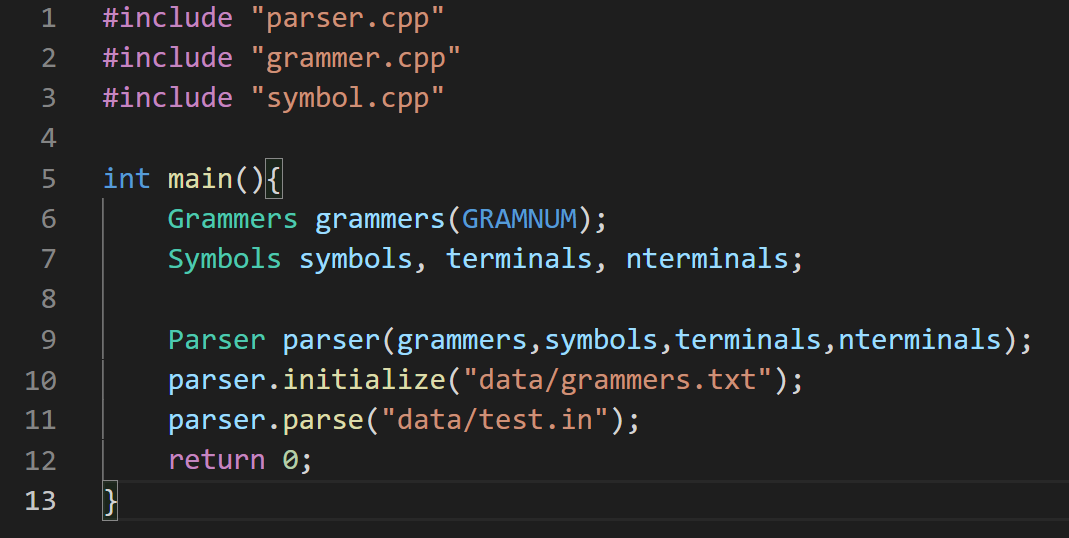
\includegraphics[width=\textwidth]{../resources/main.png}
    \end{figure}

    \subsection{和词法分析器的串联}
    需要注意的是, 实验中让设计的语法分析器是对给定的四则运算的, 那个$\mathbf{id}$根据我的理解就代表着\emph{identifier}, 也就是任何\textbf{整数, 小数, 变量};而将输入的字符串解析为有意义的符号集, 即句型, 是靠词法分析器的, 因此我将实验一的词法分析器整合到实验二中, 对每一个输入字符串, 都是\textbf{先词法分析, 再读取中间文件, 然后语法分析。}\par
    这里不得不说, 老师给的文法还是相当简单的, 如果要完成整个c--的文法, 其实应该会更复杂。\par


    \section{程序设计清单}
    如上, 我们要设计实现五个类, 其相应的成员函数, 同时要把词法分析器的内容做一些修改, 同时, 实验一我图懒省事, 所有代码放在一个.cpp文件中, 而且lexer也不是一个类, 使用函数封装的, 在整合时我就感受到了很多不方便之处, 这也是我在parser使用类的一个重要原因。\par
    更多地, 在本实验中, 我将代码组织为经典的.h声明, .cpp定义的结构, 最后在main.cpp中运行, 很优雅。

    \section{运行结果}
    将多个运算表达式写入test.in, 其中包含数字, 小数和identifier, 进行语法分析, 得到结果部分展示如\reff{fig::input}$\sim$\reff{fig::sentence1}:
    \begin{figure}[H]
        \centering
        \begin{subfigure}[b]{0.45\textwidth}
            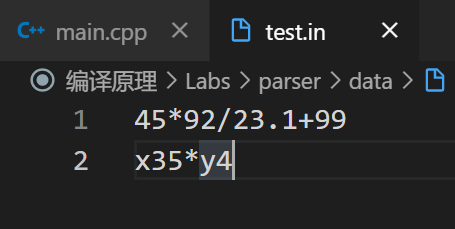
\includegraphics[width=\textwidth]{../resources/input.png}
            \caption{input}
            \label{fig::input}
        \end{subfigure}
        \begin{subfigure}[b]{0.45\textwidth}
            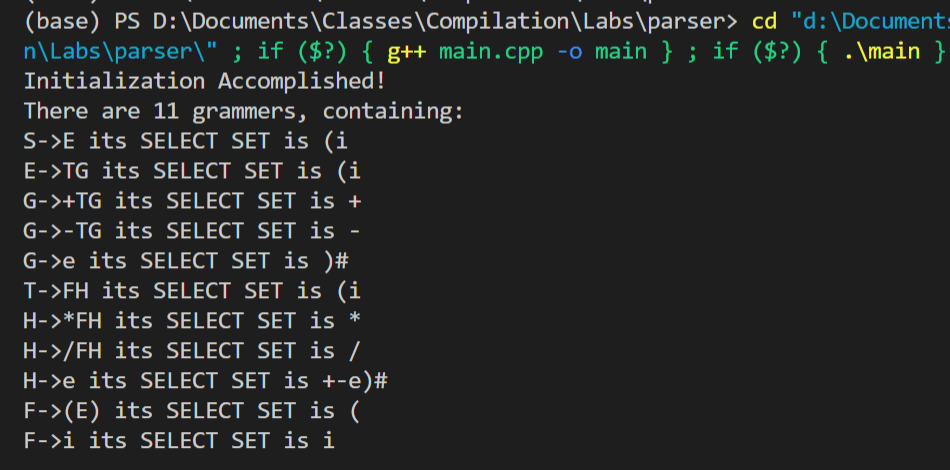
\includegraphics[width=\textwidth]{../resources/grammers.png}
            \caption{grammers}
            \label{fig::grammer}
        \end{subfigure}
        \begin{subfigure}[b]{0.4\textwidth}
            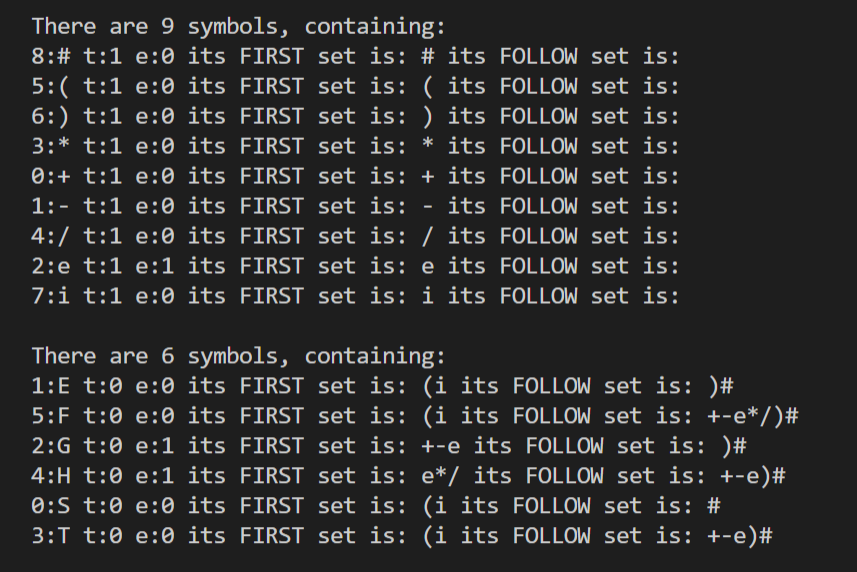
\includegraphics[width=\textwidth]{../resources/symbols.png}
            \caption{symbols}
            \label{fig::symbol}
        \end{subfigure}
        \begin{subfigure}[b]{0.4\textwidth}
            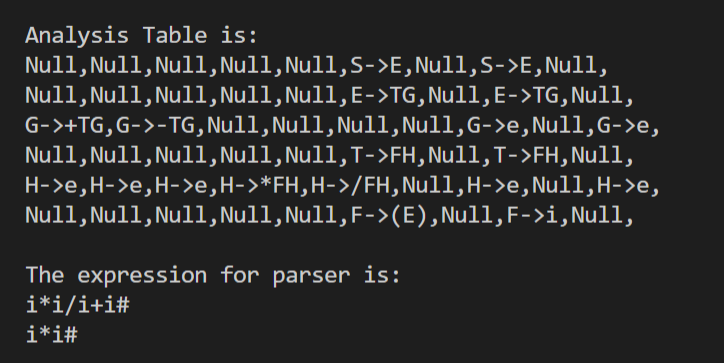
\includegraphics[width=\textwidth]{../resources/table.png}
            \caption{analysis table}
            \label{fig::table}
        \end{subfigure}
        \begin{subfigure}[b]{0.4\textwidth}
            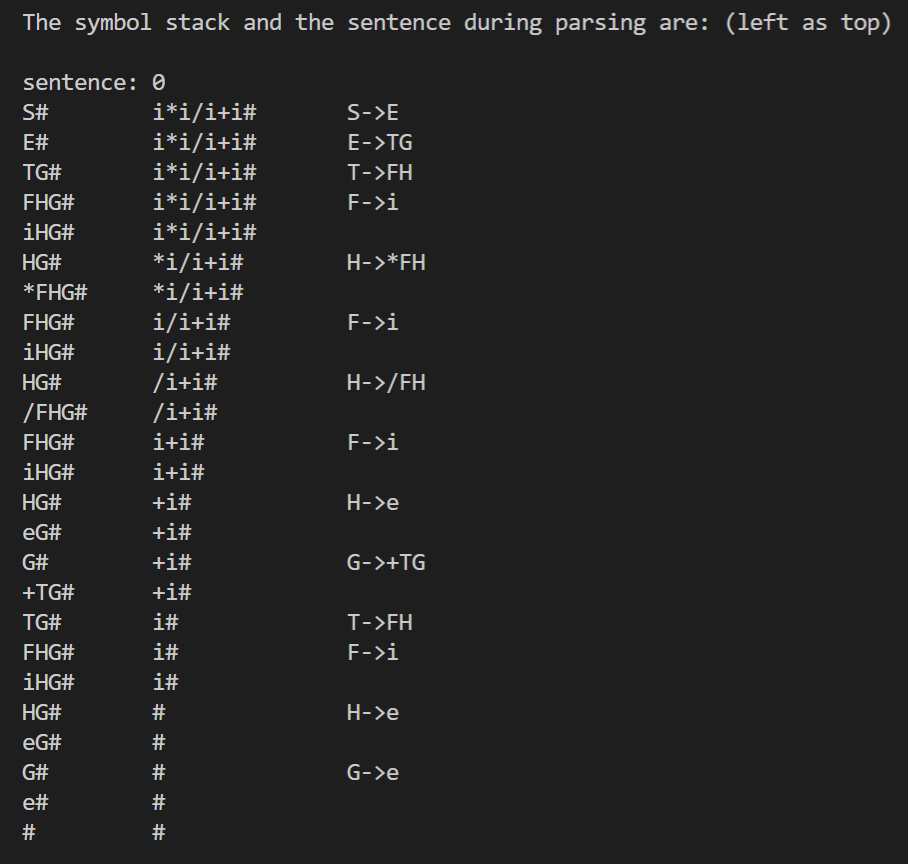
\includegraphics[width=\textwidth]{../resources/sentence0.png}
            \caption{result for the first sentence}
            \label{fig::sentence0}
        \end{subfigure}
        \begin{subfigure}[b]{0.4\textwidth}
            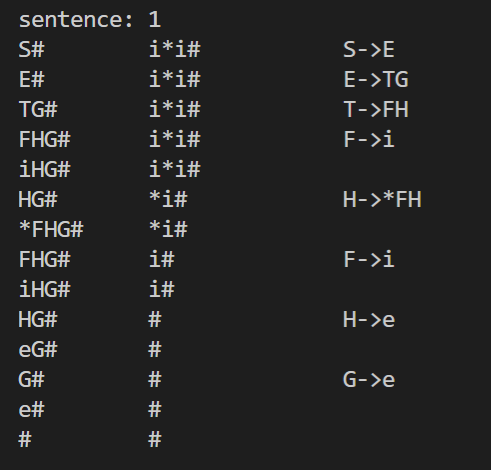
\includegraphics[width=\textwidth]{../resources/sentence1.png}
            \caption{result for the second sentence}
            \label{fig::sentence1}
        \end{subfigure}
        \caption{运行结果}
    \end{figure}
    \section{程序使用说明}
    \begin{itemize}
        \item 在data/test.in中修改要解析的字符串;
        \item 在data/grammers.txt中修改给定的文法;
        \item 在data/KeyWords.txt中修改预设关键词;
        \item 在data/Operators.txt中修改预设操作符;
        \item 在data/Separators.txt中修改预设分隔符;
        \item 语法分析的结果默认会在终端显示;
    \end{itemize}
    \section{总结与完善}
    通过这次实验, 回忆了c++的类写法, 从头到尾搞明白了LL(1)的分析逻辑, 自己完成了各项算法的设计;同时也遗留了几个问题:
    \begin{itemize}
        \item 在求某一个符号能否产生$\epsilon$时使用递归, 但是递归会将部分符号计算多次, 可以使用\textbf{动态规划}优化;
        \item 在求$\mathsf{First},\mathsf{Follow}$集时使用迭代的逻辑, 求$\mathsf{First}$要迭代4次, 求$\mathsf{Follow}$要迭代2次, 其实有很多冗余操作, 可以考虑使用递归;
    \end{itemize}
\end{document}